%%%%%%%%%%%%%%%%%%%%%%%%%%%%%%%%%%%%%%%%%%%%%%%%%%%%%%%%%%%%%%%%%%%%%%%%%%%%%%
%
% Vorlage für eine Studien- oder Diplomarbeit für den Fachbereich Informatik
% der Universität Karlsruhe (TH)
%
% Autor:   Tilo Gockel
% Version: 0.920
% Datum:   12. Mai 2010
%
% Kontakt: Hochschule Aschaffenburg,
% Tilo Gockel (Dr.-Ing.), Forschungsreferat
%
% info@formbuch.de
% http://www.formbuch.de
%
% Anmerkungen
%
% 1.) article-Style, statt report-Style
%
% Soll statt des report-Styles der article-Style genutzt werden,
% so müssen chapters durch sections, sections durch subsection usw. ersetzt
% werden. Weiterhin kann ein Kapitelbeginn auf der rechten Seite dann nicht
% mehr durch openright eingestellt werden, nur noch durch jeweilige
% \cleardoublepage -Befehle (vgl. unten).
%
%
% 2.) Lizenz
%
% Das Template darf angepasst, verändert, erweitert und auch kommerziell vertrieben werden.
% Die einzige Auflage ist, dass die Quelle des Templates in den Literaturquellen genannt
% und im Text als Quelle referenziert wird. Hierzu ist dem Text ein kurzer Satz beizufügen,
% und am Ende ist die Quelle einzufügen:
% Einzufügende Textzeile (Fußnote):
% Der vorliegende Text ist auf Basis des Latex-Templates zu [1] erstellt.
% Einzufügende zugehörige Quelle:
% [1] T. \mbox{Gockel}. Form der wissenschaftlichen Ausarbeitung. Springer-Verlag, Heidelberg, 2008.
% Begleitende Materialien unter
% \url$<http://wwwiaim.ira.uka.de/form-der-wissenschaftlichen-ausarbeitung>$.
% Weiterhin ist es sinnvoll, bei der Weitergabe des Templates die Latex-Quellen und die PDF-Datei
% nicht zu trennen.
%
%
% 3.) Versionsnummern der verwendeten Programme (alles unter Windows)
%
% (im Regelfall werden neuere Versionen aber eher von Vorteil sein)
%
%     Miktex 2.8
%     http://www.miktex.org
%
%     TexnicCenter Version 1.0 Stable Release Candidate 1
%     http://www.texniccenter.org
%
%     Texaide 4.0a
%     http://www.dessci.com/en/products/texaide
%
%     Adobe Acrobat Prof. 7.0
%     http://www.adobe.com/de/
%
%     Ghostscript 8.14, Ghostview 4.6
%     http://pages.cs.wisc.edu/~ghost
%
%     MS Office 2002, 2007 ...
%     http://office.microsoft.com/de-de/default.aspx
%
%     Adobe Photoshop CS4
%     http://www.adobe.com/de/products/photoshop/family/
%
%     Gnuplot 4.2
%     http://www.gnuplot.info
%
%     PrettyPrinter a2ps
%     http://www.gnu.org/software/a2ps
%
%     Text-Ersetzungswerkzeug grep, unter Windows
%     http://gnuwin32.sourceforge.net/packages/grep.htm
%
%
%%%%%%%%%%%%%%%%%%%%%%%%%%%%%%%%%%%%%%%%%%%%%%%%%%%%%%%%%%%%%%%%%%%%%%%%%%%%%%



\usepackage[utf8]{inputenc}   % Zeichensatz, ermöglicht die direkte Eingabe von Umlauten im Editor
\usepackage[pdftex]{graphicx} % Einbindung von Grafiken (pdf, png, jpg)
\usepackage{float}            % bietet Option [H] für bombenfestes Verankern
\usepackage[english]{babel}   % Silbentrennung nach der neuen deutschen Rechtschreibung, z.B.: Sys-tem
\usepackage{amstext}          % für Klartext via \text{} in Formeln
\usepackage{amsfonts}         % für komplexere Formeln (Mengensymbole ...)
\usepackage{amssymb}          % für komplexere Formeln (Mengensymbole ...)
\usepackage{bm}               % bold math, für \bm{}
\usepackage{enumerate}        % verbessert Aufzählungen
\usepackage[bottom]{footmisc} % Fussnoten am Seitenende
\usepackage{array}            % für Tabellen: bindet tabular-Umgebung ein
%\usepackage{algorithm}        % für Algorithmen
%\usepackage{algorithmic}      % für Algorithmen
\usepackage{ntheorem}
\usepackage{theorem}
\usepackage{pdfpages}         % für die Einbindung kompletter pdf-*Seiten*
\usepackage{parskip}          % zw. Absätzen: eine knappe Leerzeile statt hängender Einzüge
\usepackage[right]{eurosym}   % Eurosymbol
%\usepackage{xcolor}           % farbiger Text
%\usepackage{colortbl}
\usepackage{xcolor}
\usepackage{tabu}
%\usepackage[hyphens]{url}     % für \url{http://www}, Option hyp erlaubt auch Umbruch nach "-"
\usepackage{makeidx}          % Package zur Indexerstellung
\usepackage{multicol}         % zur Indexerstellung in zwei Spalten
% \usepackage[numbers, square]{natbib}   % Für \setlength{\bibsep}{3mm}; square macht eckige Klammern
\usepackage{csquotes}
\usepackage[
  style=numeric,
  backref,
  backend=biber,
  defernumbers=true,
  useprefix=true,
  giveninits=true,
  maxbibnames=99, minbibnames=99,
  sorting=none
]{biblatex}
\usepackage[T1]{fontenc}
\usepackage{hyperref}
%\usepackage{tabularx}
\usepackage{caption}
\usepackage[printonlyused]{acronym}
\usepackage{listings}
\usepackage{chngcntr}

\usepackage{tikz}
\usetikzlibrary{fit}

\usepackage[chapter]{minted}
\setminted{
  breaklines,
  frame=lines,
  linenos,
  python3=true,
  style=manni,
  xleftmargin=0.6cm
}

\usepackage{settings/chapterthumb}
\usepackage{wrapfig}

\counterwithout{figure}{chapter}
\counterwithout{table}{chapter}

\captionsetup[table]{skip=10pt}

\NeedsTeXFormat{LaTeX2e}            % Unklar, gehoeren aber zusammen:
\ProvidesPackage{hyperref}          % http://janeden.net/eigene-dokumentklassen
\hypersetup{
  pdftex=false,
  colorlinks=true,
  breaklinks=true,
  linkcolor=black,
  menucolor=black,
  urlcolor=black,
  citecolor=black
}


%\usepackage[cmex10]{amsmath}  % für erw. Formeloptionen, Option [] zur Vermeidung von Type3-Fonts
%\usepackage{mathcomp}         %\tcmu \tcohm \tccelsius.. im Mathemodus, nichtkursiv; problematisch!
%\usepackage{textcomp}         % für \textdegree , \textcelsius , macht aber manchmal auch Probleme!


%\usepackage[plainpages=false, hypertexnames=false]{hyperref}
                               % hyperref statt \url geht, verträgt sich allerdings nicht mit den
                               % eingefügten / veränderten Seitenzahlen ... (die stimmen dann nicht mehr)



\definecolor{darkred}{rgb}{0.7,0.0,0.0}
\definecolor{dunkelgrau}{rgb}{0.8,0.8,0.8}
\definecolor{hellgrau}{rgb}{0.92,0.92,0.92}
\definecolor{fgcgray}{rgb}{0.4, 0.4, 0.4}
\definecolor{bgctitle}{rgb}{0.5, 0.5, 0.5}
\definecolor{fgctitle}{rgb}{0.95, 0.95, 0.95}
\definecolor{lightgreen}{RGB}{219, 249, 189}
\definecolor{lightred}{RGB}{255, 204, 203}
\definecolor{fullred}{RGB}{255, 0, 0}

\definecolor{ob_dark_gray}{HTML}{58585a}
\definecolor{ob_light_gray}{HTML}{a5a5a6}
\definecolor{ob_orange}{HTML}{ea9023}

\renewcommand{\figurename}{Fig.}
\renewcommand{\tablename}{Tab.}
\newcommand{\sectionname}{Sec.}
\newcommand{\equationname}{Eq.}
\renewcommand{\lstlistlistingname}{List of Listings}

\newcommand{\todo}[1]{{{\color{fullred}#1}}}

\sloppy                       % großzügiger Zeilenumbruch
                              % -> keine rechts rausragenden Zeilen mehr


%%%%%%%%%%%%%%%%%%%%%%%%%%%%%%%%%%%%%%%%%%%%%%%%%%%%%%%%%%%%%%%%%%%%%%%%%%%%%%
%
% Index-Erstellung
%
% Anmerkung: für die Indexerstellung muss auch die TeXnicCenter-IDE angepasst
% werden:
% 1.) Projekt / Eigenschaften / verwendet MakeIndex [x]
% 2.) Ausgabe / Ausgabeprofil definieren
%
\makeindex % erstelle einen Index bzw. ein Sachverzeichnis)
%
% Wenn kein Index gewünscht ist: einfach \makeindex auskommentieren
%
%%%%%%%%%%%%%%%%%%%%%%%%%%%%%%%%%%%%%%%%%%%%%%%%%%%%%%%%%%%%%%%%%%%%%%%%%%%%%%



%%%%%%%%%%%%%%%%%%%%%%%%%%%%%%%%%%%%%%%%%%%%%%%%%%%%%%%%%%%%%%%%%%%%%%%%%%%%%%
%
% Größenanpassungen
%
\setlength{\unitlength}{1cm}
\setlength{\oddsidemargin}{0.3cm}
\setlength{\evensidemargin}{0.3cm}
\setlength{\textwidth}{15.5cm}
\setlength{\topmargin}{-1.2cm}
\setlength{\textheight}{23cm}
\columnsep 0.5cm
%
%%%%%%%%%%%%%%%%%%%%%%%%%%%%%%%%%%%%%%%%%%%%%%%%%%%%%%%%%%%%%%%%%%%%%%%%%%%%%%



%%%%%%%%%%%%%%%%%%%%%%%%%%%%%%%%%%%%%%%%%%%%%%%%%%%%%%%%%%%%%%%%%%%%%%%%%%%%%%
%
% Beispiel für die Anpassung des Satzspiegels und
% die Verwendung von Schnittmarken (momentan ausgeschaltet)
% Im Beispiel: Anpassung des Drucks auf Taschenbuchformat
%
% Obacht: für Tests hiermit (Probeausdrucke...):
% stets im Adobe Acrobat im Druckdialog die Seitenanpassung *abschalten*!
% sonst stimmen die Maße nicht!
%
%
%\usepackage[total={90mm,144mm},centering]{geometry}
%\geometry{papersize={120mm,190mm}}
%\usepackage[a4,cam,center]{crop}
%\crop[]
%
% Schnittmarken und Satzspiegel - Ende
%
%%%%%%%%%%%%%%%%%%%%%%%%%%%%%%%%%%%%%%%%%%%%%%%%%%%%%%%%%%%%%%%%%%%%%%%%%%%%%%



%%%%%%%%%%%%%%%%%%%%%%%%%%%%%%%%%%%%%%%%%%%%%%%%%%%%%%%%%%%%%%%%%%%%%%%%%%%%%%
%
% Abkürzungsliste, Liste explizit vorgegebener Abk.
%
% Anmerkung: für Wörter mit Umlauten
% muss das Paket \usepackage[T1]{fontenc} eingebunden werden --
% in der vorliegenden Version funktionieren *keine* Umlaute!!
%
\hyphenation{Da-tei-grö-ßen-be-schränk-ung Au-then-ti-fi-zier-ung Ent-wick-ler-apps Ent-wick-ler-app Hash-funk-tion-en Ver-schlüs-sel-ungs-algo-rith-mus}
%
%%%%%%%%%%%%%%%%%%%%%%%%%%%%%%%%%%%%%%%%%%%%%%%%%%%%%%%%%%%%%%%%%%%%%%%%%%%%%%


\usepackage[nohints]{minitoc}                 % ToC for chapters
\dominitoc[n]                                 % ToC: no caption
\renewcommand{\mtcSfont}{\small}              % ToC: small
\usepackage{makeidx}                          % Make an index
\makeindex                                    % Make an index

\newcommand{\doit}{\begin{figure}[H]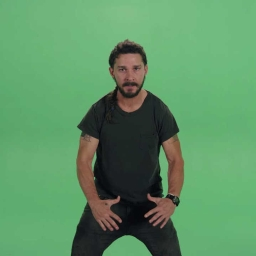
\includegraphics[width=0.2\textwidth]{resources/images/do_it.jpg}\end{figure}}
